\subsection{The \texttt{no-coalescence.h} algorithm}

In previous studies various methods have been used to avoid coalescence. 
One method is to increase artificially the surface tension coefficient at the interface points, as demonstrated in the recent study of \citet{hidman2023assessing}.
This method seems highly efficient, in terms of simplicity and computational expenses. However, it remains unclear if the physical behavior of the droplets interactions is well captured due to the introduction of artificial forces. 
Additionally, its applicability for denser emulsion, up to $\phi = 0.2$, remains uncertain. 
On another hand, in \citet{balcazar2015multiple} they developed a multiple marker level-set method to prevent coalescence, while \citet{zhang2021direct} utilized a Multi-VoF method. 
The latter method consists in assigning to each droplet a different color function, so  that the interfaces are properly reconstructed when droplets are in close contact.
In turns, droplets in contact never coalesce.  
The latter method may be suitable for our objectives. 
However, it can be quite expensive as it requires solving a transport equation for each tracer, with one tracer assigned per droplet, meaning $125$ tracer in our case. 
In \citet{karnakov2022computing} they developed a Multi-VoF method which requires a fixed number of tracers for an arbitrary number of droplets.
% Instead, we adopt the methodology proposed by \citet{karnakov2022computing} which consider a number of tracers independent of the number of droplets.
This approach allows multiple non-touching droplets to belong to the same field, which makes it more efficient than the previous study.
Although this approach shares the same basic principle with the one used here, i.e. we color adjacent droplets with different colors to avoid coalescence, it differs in terms of computational methods. 
Therefore, in the following we present our methodology that is implemented in the \texttt{Basilisk} code. 

The challenge here is to assign a tracer to every adjacent droplets to prevent numerical coalesce, while minimizing the number of tracers to reduce computational costs. 
This recall the famous \textit{Four color map theorem} \citep{appel1977solution} which essentially states that : 
\enquote{every map can be color using only four colors, so that two neighboring region are different colors}. 
In our case, this theorem implies that for any 2D configuration only four VoF tracer are necessary to avoid coalescence\footnote{It's worth noting that on a bi-periodic domain, seven colors are required due to the periodic boundary condition, which gives the domain a torus-like topology  }. 
Therefore, leveraging \textit{Four color map theorem}, one might be able to significantly reduce the number of VoF tracers required.
Nevertheless, the optimal coloring problem is originally a static planar coloring problem that need to be solved once. 
However, in our case, droplets may move around over time, transforming the static problem into a time-dependent planar problem. 
Thus, even if a solution exists in 2D configuration, these problems are theoretically expensive to solve (NP-complete), and even more so if they must be solved at each time step.  
In the three-dimensional space the \textit{Four color map theorem} has no equivalent. 
% One of them is shown \ref{fig:colors}, where five 3 dimensional objects all touch each other so that five color is needed. 
For example, an arbitrary large number of rectangular blocks in the 3D spaces can all touch each other, requiring an arbitrary large number of colors to differentiate the adjacent blocks\citep{magnant2011coloring}. 
% \begin{figure}
%     \centering
%     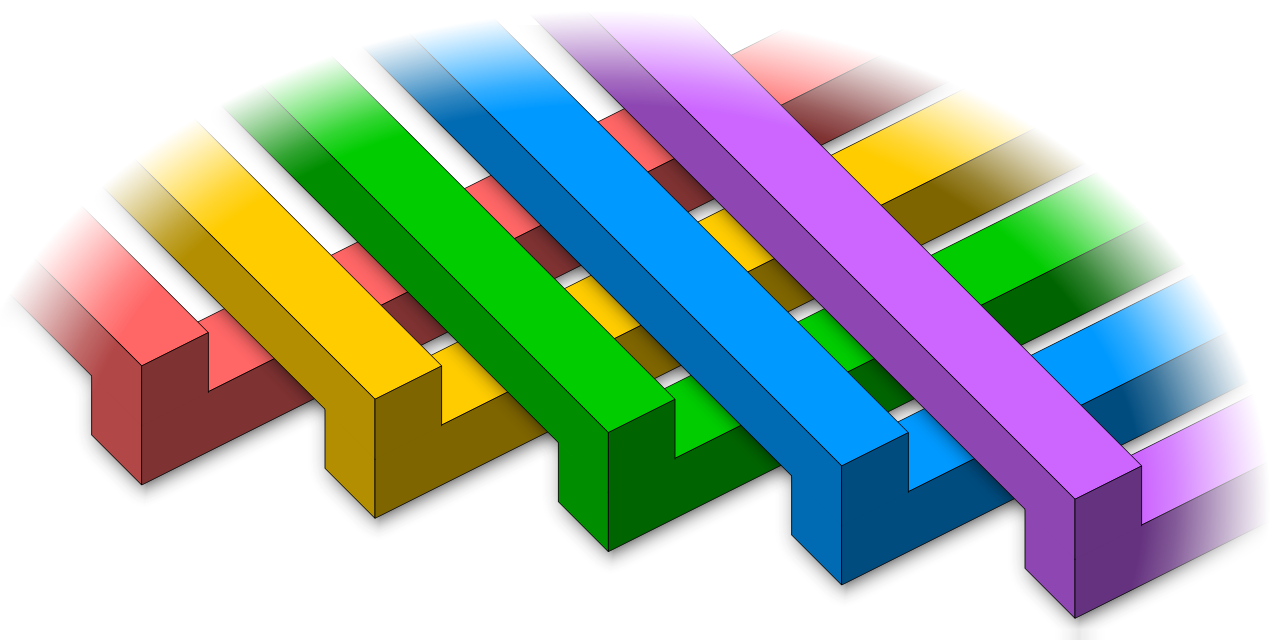
\includegraphics[width=0.5\textwidth]{image/more_than_four.png}
%     \caption{
%     Proof of the non validity of the \textit{Four color map theorem} in three-dimensional spaces. 
%     3 dimensional pictures of five regions all touching each other. 
%     Clearly, in this case 5 color is required. 
%     }
%     \label{fig:colors}
% \end{figure}
From the knowledge of the author no such problem has been solved for 3D spheres. 
Nevertheless, it is reasonable to assume that the number of tracers required to avoid coalescence is significantly fewer than the number of droplets.
Consequently, since we cannot determine the optimal coloring configuration based on theoretical grounds, we opt to assign the tracers to each droplet following the empirical strategy detailed below.

The development of the \texttt{no-coalesce.h} algorithm was initiated in the PhD. thesis of \citet{mani2021numerical}.
The latest version of this algorithm (as of the current date), can be found on the basilisk wiki page : \href{http://basilisk.fr/sandbox/fintzin/Rising-Suspenion/no-coalescence.h}{no-coalescence.h}.
Before  diving into a step-by-step description of this algorithm we need to introduce another key feature used in these simulations, which is the \href{http://basilisk.fr/src/tag.h}{tag.h} algorithm. 
It is an adaptation of the \textit{painter’s} algorithm, but optimized using the multigrid solver. 
Its purpose is to assign different scalars values to each cell belonging to different regions, with the regions being delimited by the different droplets' interfaces. 
For instance, on \ref{fig:images} (left) we can observe two blue regions corresponding to two different drops.
We can note that both are assigned with two different values, $1$ and $2$, which are identified using the \texttt{tag.h} algorithm. 
Then, it is straightforward to obtain a droplet's properties, such as its center of mass position and velocity, by carrying numerical integration on the VoF field considering only the cells having a specific tag value, which corresponds to a given droplet.  
In general, we are able to differentiate droplets' domain, belonging to the same tracer thanks to the \texttt{tag.h} algorithm. 

We define the $i^\text{th}$ color function as $C_i$ for $i =1,2,\ldots,N(t)$, where $N(t)$ is the total number of tracers used in a simulation at time $t$.
The color function introduced previously is now defined as, $C = \sum_{i=1}^{N(t)} C_i$. 
Note that $N(t)$ is time dependent since the number of tracer might increase along the simulation time as the droplets get in contacts. 
The simplified workflow of the algorithm follows these four steps : 
\begin{enumerate}
    \item[\textit{Step 1}.] Check if within a tracer field $C_i$, the droplets are possibly too close to each other. 
    The \textit{near contact} criterion that determine if the droplets are too close, is defined such that we iterate a $5$ by $5$ cells stencil which verifies the following condition : 
    (1) If the color function $C_i = 0$ at the center of the stencil. 
    (2) And if $C_i > 1$ for two opposite cells in the stencil. 
    In which case two different regions might be in close contact.
    A scheme of this situation is given in \ref{fig:criterion}.  
    \item[\textit{Step 2}.] 
    If (\textit{Step 1}.) is true for the tracer $C_i$, we must verify if we indeed identified two different regions in near contact, and not just a single region that merge into itself, such as in \ref{fig:diagram} (right). 
    Therefore, at this step  we apply the \texttt{tag.h} algorithm.
    \item[\textit{Step 3}.] Re-use the \textit{near contact} criterion of (\textit{Step 1}.) by requiring in addition that the cells must belong to two different tags groups. 
    % In which case we are sure that we are in presence of two cells belonging to the same tracer but not to the same drops, and that both region are in near contact.
    At this stage the situation in \ref{fig:criterion} (left) would be true, while the situation on \ref{fig:criterion} (right) would be false. 
    We therefore identified all the droplets / region that are indeed too close to each other. 
    \item[\textit{Step 4}.] 
    Find a new tracer field $C_n$, in which we could set the region/droplets that are in near contact. 
    At this stage, it's essential to identify the list of tracer $C_j$ already in contact with the region to be replaced. 
    For example, in \ref{fig:criterion} (left), the droplet on the right is clearly adjacent to a region with tracer $C_j$, in which case $C_n$ must satisfy $n \neq i,j$. 
    Therefore, any $n$ in $1, 2, \ldots, N(t)$ are suitable candidates as long as this situation is avoided. 
    If the droplet is already adjacent to every tracer $C_j$ in the simulation, for $j = 1, 2, \ldots, N(t)$, we create a new tracer $C_n$ with $n = N(t)+1$ and assign the drop to this tracer field.
\end{enumerate}
\begin{figure}
    \centering
    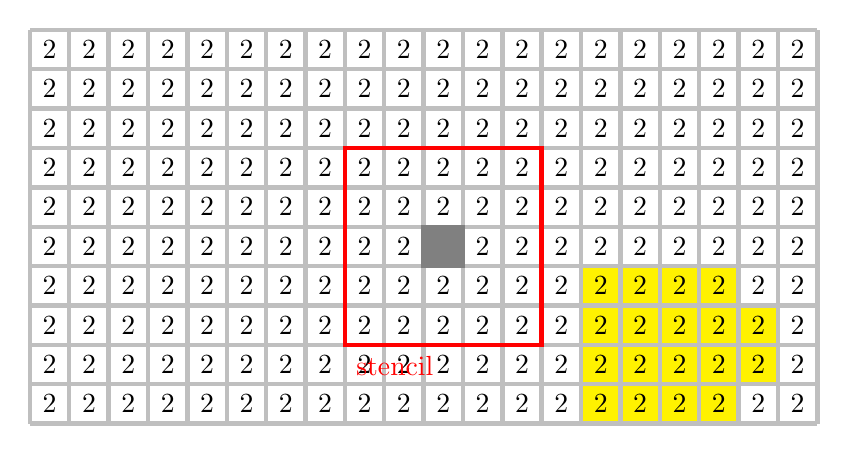
\begin{tikzpicture}[scale=0.5,ultra thick]
        % Define grid dimensions
        \def\nRows{10}
        \def\nCols{20}
        \pgfmathsetmacro\nRowsm{\nRows-1}
        \pgfmathsetmacro\nColsm{\nCols-1}

        \foreach \row in {0,...,\nRowsm} {
            \foreach \col in {0,...,\nColsm} {
                \pgfmathsetmacro\distance{veclen(\col-4.356, \row-2.65)};
                \pgfmathparse{\distance < 4 ? "blue" : "white"}
                \edef\colour{\pgfmathresult};
                \ifthenelse{\equal{\colour}{blue}}{                    
                    \fill[\colour!60!white] (\col, \row) rectangle ++(1,1);
                    \node (num) at (\col +0.5,\row+0.5){1};
                }
            }
        }

        \foreach \row in {0,...,\nRowsm} {
            \foreach \col in {0,...,\nColsm} {
                \pgfmathsetmacro\distance{veclen(\col-15, \row-6.2)};
                \pgfmathparse{\distance < 3.5 ? "blue" :"white"}
                \edef\colour{\pgfmathresult};
                \ifthenelse{\equal{\colour}{blue}}{
                    \fill[\colour!60!white] (\col, \row) rectangle ++(1,1);
                \node (num) at (\col +0.5,\row+0.5){2};
                }
            }
        }

        \foreach \row in {0,...,\nRowsm} {
            \foreach \col in {0,...,\nColsm} {
                \pgfmathsetmacro\distance{veclen(\col-15.62, \row-1.5)};
                \pgfmathparse{\distance < 2.5 ? "yellow" :"white"}
                \edef\colour{\pgfmathresult};
                \ifthenelse{\equal{\colour}{yellow}}{
                    \fill[\colour] (\col, \row) rectangle ++(1,1);
                    \node (num) at (\col +0.5,\row+0.5){2};
                }
            }
        }
        % Define grid size
        \pgfmathsetmacro\gridSize{1}
        
        \foreach \row in {0,...,\nRows} {
            \draw [gray!50] (0,\row*\gridSize) -- (\nCols*\gridSize,\row*\gridSize);
        }
        % Draw vertical grid lines
        \foreach \col in {0,...,\nCols} {
            \draw [gray!50] (\col*\gridSize,0) -- (\col*\gridSize,\nRows*\gridSize);
        }
        % Draw drop shape
        \draw[red] (8,2)node[below right]{stencil} rectangle +(5,5); % Draw the rectangular base
        \filldraw[gray] (10,4) rectangle +(1,1);
    \end{tikzpicture}    
    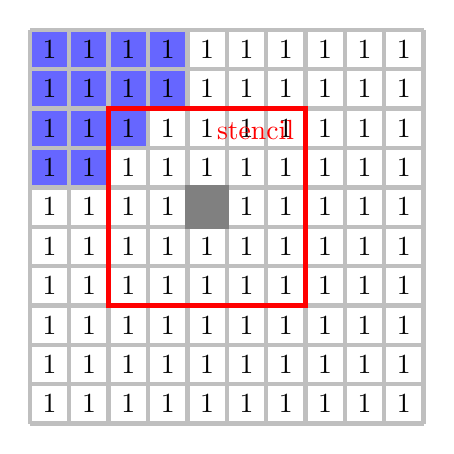
\begin{tikzpicture}[scale=0.5,ultra thick]
        % Define grid dimensions
        \def\nRows{10}
        \def\nCols{10}
        \pgfmathsetmacro\nRowsm{\nRows-1}
        \pgfmathsetmacro\nColsm{\nCols-1}

        \foreach \row in {0,...,\nRowsm} {
            \foreach \col in {0,...,\nColsm} {
                \pgfmathsetmacro\distance{veclen(\col, \row-2)};
                \pgfmathparse{\distance < 3.5 ? "blue" :"white"}
                \edef\colour{\pgfmathresult};
                \ifthenelse{\equal{\colour}{blue}}{
                    \fill[\colour!60!white] (\col, \row) rectangle ++(1,1);
                \node (num) at (\col +0.5,\row+0.5){1};
                }
            }
        }

        \foreach \row in {0,...,\nRowsm} {
            \foreach \col in {0,...,\nColsm} {
                \pgfmathsetmacro\distance{veclen(\col-7, \row-2)};
                \pgfmathparse{\distance < 3.5 ? "blue" :"white"}
                \edef\colour{\pgfmathresult};
                \ifthenelse{\equal{\colour}{blue}}{
                    \fill[\colour!60!white] (\col, \row) rectangle ++(1,1);
                    \node (num) at (\col +0.5,\row+0.5){1};
                }
            }
        }
        \foreach \row in {0,...,\nRowsm} {
            \foreach \col in {0,...,\nColsm} {
                \pgfmathsetmacro\distance{veclen(\col-5, \row)};
                \pgfmathparse{\distance < 3.5 ? "blue" :"white"}
                \edef\colour{\pgfmathresult};
                \ifthenelse{\equal{\colour}{blue}}{
                    \fill[\colour!60!white] (\col, \row) rectangle ++(1,1);
                    \node (num) at (\col +0.5,\row+0.5){1};
                }
            }
        }
        \foreach \row in {0,...,\nRowsm} {
            \foreach \col in {0,...,\nColsm} {
                \pgfmathsetmacro\distance{veclen(\col, \row-9)};
                \pgfmathparse{\distance < 3.5 ? "blue" :"white"}
                \edef\colour{\pgfmathresult};
                \ifthenelse{\equal{\colour}{blue}}{
                    \fill[\colour!60!white] (\col, \row) rectangle ++(1,1);
                    \node (num) at (\col +0.5,\row+0.5){1};
                }
            }
        }
        % Define grid size
        \pgfmathsetmacro\gridSize{1}
        
        \foreach \row in {0,...,\nRows} {
            \draw [gray!50] (0,\row*\gridSize) -- (\nCols*\gridSize,\row*\gridSize);
        }
        % Draw vertical grid lines
        \foreach \col in {0,...,\nCols} {
            \draw [gray!50] (\col*\gridSize,0) -- (\col*\gridSize,\nRows*\gridSize);
        }
        % Draw drop shape
        \draw[red] (2,3) rectangle +(5,5)node[below left]{stencil}; % Draw the rectangular base
        \filldraw[gray] (4,5) rectangle +(1,1);
    \end{tikzpicture}    
    \caption{Scheme of two situations were the \textit{near contact} criterion is true. 
    The background grid represents the cells within the numerical domain. 
    The dark blue area represents the cells where $C_i > 0$.
    The yellow area represents the cells where the tracer $C_j > 0$ for $j\neq i$. 
    The numbers represent the value of the $Tag$ scalar fields within each tracer.
    The $5$ by $5$ cells red rectangle represent the stencil zone which iterate over all cells of the domain.  
    %  where the center of the stencil (gray square) must respect $C_i = 0$. 
    (left) Two droplets in contact since we have two opposite cells in the stencil with $C_i > 0$ and $C_i=0$ at the center.
    And, the mentioned cells belong to two different regions so that (\textit{Step 3}) is also validated.  
    (right) A near contact is observed since we have two opposite cells in the stencil with $C_i > 0$ and $C_i=0$ at the center, however in this case we do not complete the second criterion of \textit{Step 3} which require two different tags values. 
    }
    \label{fig:criterion}
\end{figure}
These four steps are executed at each simulation time step and for each tracer $C_i$ with $i = 1, 2, \ldots, N(t)$.
Following this procedure, we ensure that all adjacent droplets belong to different tracers, which ultimately prevents coalesce to happen. 

Having $N(t)$ tracers requires some modifications to the aforementioned governing equations. 
Specifically, instead of solving \ref{eq:dt_C}, we solve $N(t)$ transport equations, one for each $C_i$.
Likewise, the surface tension force is computed as the sum of the contributions from each $C_i$.
It reads,  
\begin{align*}
    \pddt C_i + \textbf{u}\cdot\grad C_i = 0,
    \ \  \ \ \forall i = 1,2,\ldots N(t),\\
    \textbf{f}_\gamma 
    = \sum_{i=0}^{N(t)} \gamma \kappa_i \grad C_i
\end{align*}
where $\kappa_i$ is the numerical approximation of the curvature of the interface of the field $C_i$, which is computed following the same method employed for a single tracer. 

\ref{fig:diagram} (left) shows a snapshot of a simulation at an arbitrary time $t^* = 100 \sqrt{g/d}$. 
The droplets' interface is colored by the indices of their respective tracer. 
In this simulation at that time, no more than 3 colors are needed to avoid coalescence.
On \ref{fig:diagram} (right) we display the value of $N(t)$ in terms of the dimensionless simulation time for various volume fraction $\phi$ at $Ga = 50$ and  $\lambda = 1$. 
We observe that for the entire simulation, no more than 3 tracers were needed for the dilute emulsion ($\phi = 0.01$), up to 7 for the denser regime ($\phi = 0.2$). 
Although our algorithm might not be optimized, it brings sufficient efficiency for our needs. 
Indeed, \ref{tab:performance} report all the time spent by each functions during a simulation. 
It is observed that the \texttt{no-coalesce.h} algorithm accounts for approximately $4\%$ of the total computational time of a simulation. 
As for the \texttt{tag.h} algorithm, its cost is around $2\%$, which is also considered reasonable.
In comparison, the \texttt{poisson.h} solver is about $13\%$ of the simulation time. 
Regarding, the advection of VoF tracers it is about $7\%$, due to the presence of several VoF tracer. 
Anyhow, we believe that further developments, which are referenced at \href{http://basilisk.fr/sandbox/fintzin/Rising-Suspenion/no-coalescence.h}{no-coalescence.h}, might be useful for future studies.\tb{mettre latodo list}
\begin{figure}[h!]
    \centering
    \begin{tikzpicture}
    \node (img) at (0,0) {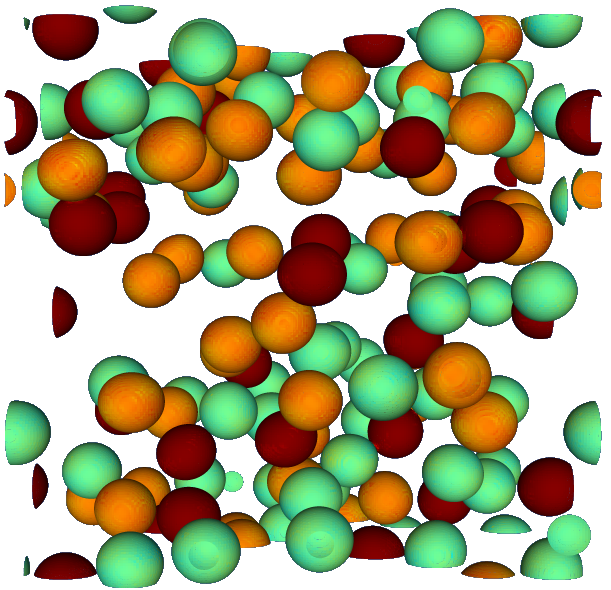
\includegraphics[width = 0.4\textwidth]{image/VoF2.png}};
    \node (img) at (0.4\textwidth,-0.01\textwidth) {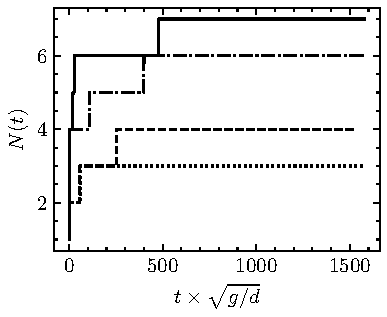
\includegraphics[width = 0.4\textwidth]{image/HOMOGENEOUS_NEW/CA/NVoF_vs_t_Ga_50_l_1.pdf}};
    \end{tikzpicture}
    \caption{
    (left) Snapshot of a DNS with $\phi = 0.05$, $\lambda = 1$, $Ga = 50$ with the interface of the droplets colored by the index of the tracer.
    (right) Number of tracer $N(t)$, in terms of the dimensionless time.
    Four different volume fractions are displayed : (dotted line) $\phi = 0.01$, (dashed line) $\phi = 0.05$ (dash dotted line) $\phi = 0.1$ (solid line) $\phi = 0.2$ at $Ga = 50$ and $\lambda = 1$. 
    }
    \label{fig:diagram}
\end{figure}

With a grid resolution of $\Delta/d = 30$, the film between the droplets that are in close contact is not resolved. 
Therefore, the question arises: How accurate is the dynamic of interaction at the droplet scale?
Answers are  provided in \ref{ap:validation} (\textit{Case 2.}) where we compare our DNS to \citet{mohamed2003drop} experiments.
In \citet{mohamed2003drop} they experimentally study the impact of a single drop on a flat interface of the same fluid, while recording the positions of the interfaces.
It is found that the Multi-VoF method captures remarkably well the position of interfaces, even with a poor description of the liquid film between these interfaces.
Nevertheless, these experiments were performed at $Bo = 6$, which is significantly higher than $Bo=0.2$ used in this work. 
When two droplets approach each other, viscous dissipation is generated within the liquid film present between two droplets' interfaces.
This dissipation occurs until that the droplets' interfaces deform.
Thus, for rigid interfaces, meaning low \textit{Bond} number, we expect more viscous dissipation within the film compared to deformable interfaces. 
Therefore, it is likely that at $Bo = 0.2$, more viscous dissipation are present within the film during a collision.
This might lead to a larger error in our simulations since we do not solve the flow in the film, and neglect this larger viscous dissipation.
Nevertheless, we argue that the mesh independence study conducted in \ref{ap:validation} (Case 3) substantiates the accuracy of the DNS, as the dynamics of interaction do converge with  reasonable errors for a grid resolution of $\Delta/d = 30$.
Overall, we used an optimized Multi-VoF method, enabling us to perform DNS with a maximum of 7 tracers in the densest scenario.
 





